\documentclass[a4paper,11pt]{article}
\usepackage[margin=20mm]{geometry}
\usepackage{amsmath,amssymb,graphicx,booktabs,array,float,hyperref}
\hypersetup{hidelinks}
\setlength{\parindent}{0pt}
\setlength{\parskip}{5pt}
\renewcommand{\arraystretch}{1.14}
\setlength{\tabcolsep}{4pt}
\begin{document}
\thispagestyle{empty}
\begin{center}{\Large\bfseries Beihang University\\School of Mathematical Sciences\\Laboratory Report}\end{center}
{\small Detailed derivations, results and analysis continue on the following pages.}\par
\vspace{3mm}
\begin{tabular}{|p{.22\linewidth}|p{.22\linewidth}|p{.22\linewidth}|p{.22\linewidth}|}\hline
\multicolumn{2}{|p{.47\linewidth}|}{Course: Numerical Analysis Computer Laboratory} & \multicolumn{2}{p{.43\linewidth}|}{GMRES for Large Sparse Linear Systems}\\\hline
\multicolumn{4}{|l|}{Experiment type: Demonstration [ ] Verification [ ] Comprehensive [ ] Design [ ]}\\\hline
Class: 230116 & \multicolumn{2}{l|}{Name: yule yang} & Student ID: 23376268\\\hline
Lab date: 2026.10.17 & \multicolumn{2}{l|}{Instructor:} & Grade:\\\hline

\multicolumn{4}{|p{.95\linewidth}|}{\textbf{Experimental environment}\par macOS on Apple Silicon; Python with NumPy and SciPy; Matplotlib for plots. AI assistance: Codex. Exact package versions and measured results are archived with the experiment.\par\vspace{4mm}}\\\hline
\multicolumn{4}{|p{.95\linewidth}|}{\textbf{Objectives and content}\par Solve the three supplied sparse systems with Gauss Seidel, restarted GMRES and ILU GMRES. Solve the boundary value problem on grids of 50, 100 and 200 subintervals. Compare true residuals, solution errors, time and convergence order.\par\vspace{4mm}}\\\hline
\multicolumn{4}{|p{.95\linewidth}|}{\textbf{Procedure and results}\par All six prescribed cases were run. Gauss Seidel diverges for Experiment 1.2. All GMRES and ILU GMRES runs meet the true relative residual target of 1e-11. The finite difference solution exhibits second order convergence.\par\vspace{4mm}}\\\hline
\multicolumn{4}{|p{.95\linewidth}|}{\textbf{Analysis and conclusions}\par ILU reduces iteration counts substantially on these sparse matrices. Timings include monitoring and depend on this implementation and machine. Discretization error and algebraic solver error are assessed separately.\par\vspace{4mm}}\\\hline
\end{tabular}
\clearpage
\section*{1 Methods and matrix conventions}
The three supplied linear systems use the exact solution consisting entirely of ones; their right hand sides are formed by sparse multiplication. All solvers start at zero and use the same true relative residual stopping target. The implementation is compared with SciPy GMRES and a sparse direct solve. No dense matrix inverse is formed.

\[r_k=b-Ax_k,\qquad \frac{\|r_k\|_2}{\|b\|_2}\leq 10^{-11},\qquad e_k=\|x_k-x_*\|_2.\]
\subsection*{Stationary iteration and Krylov minimization}
\[A=D+L+U,\qquad (D+L)x_{k+1}=b-Ux_k.\]
Gauss Seidel uses a sparse triangular solve per sweep. Divergence is reported when the residual exceeds its initial value by a factor of 1e12. Restarted GMRES uses 30 Arnoldi vectors, two modified Gram Schmidt passes, and a small least squares solve at each inner iteration. The iteration cap is 10000 for both algorithms.

\[AM^{-1}V_k=V_{k+1}\overline{H}_k,\qquad x_k=x_{\mathrm{base}}+M^{-1}V_ky_k.\]
\[y_k=\arg\min_y\|\beta e_1-\overline{H}_ky\|_2,\qquad \beta=\|b-Ax_{\mathrm{base}}\|_2.\]
The teaching code applies right preconditioning: M is the incomplete LU factorization and M inverse is applied by triangular solves. Unpreconditioned GMRES uses the identity. ILU uses drop tolerance 1e-4, fill factor 10 and natural ordering. SciPy uses its own left preconditioned interface; both implementations are compared using the original residual and final solution, rather than requiring identical iteration histories.

\subsection*{Measurement protocol}
Five independent repeats are timed per method and case. Tables report the median total time including ILU setup, triangular splitting and all residual/error sampling. Curves show solve time only, from the repeat whose total time is the median. Python overhead and repeated least squares solves influence the measured ranking; these are laboratory timings, not a benchmark of optimized implementations.

\clearpage
\section*{2 Experiment 1.1 results}
The 300 by 300 tridiagonal matrix has diagonal 61.0001, lower diagonal 35 and upper diagonal 25. Its rows are strictly diagonally dominant because 61.0001 exceeds 35 + 25. This supports Gauss Seidel convergence. The asymmetry is retained exactly.

\[A_{ii}=61.0001,\quad A_{i,i-1}=35,\quad A_{i,i+1}=25,\quad b=A\mathbf{1}.\]
{\small\begin{tabular}{p{0.182\linewidth}p{0.182\linewidth}p{0.182\linewidth}p{0.182\linewidth}p{0.182\linewidth}}\toprule
Method & Iterations & Relative residual & Error norm & Total ms\\\midrule
Gauss-Seidel & 326 & 9.745e-12 & 1.960e-08 & 44.3508\\
GMRES & 192 & 9.817e-12 & 1.432e-08 & 15.5926\\
ILU-GMRES & 1 & 9.840e-17 & 6.435e-15 & 0.1112\\
\bottomrule\end{tabular}}\par
\begin{figure}[H]\centering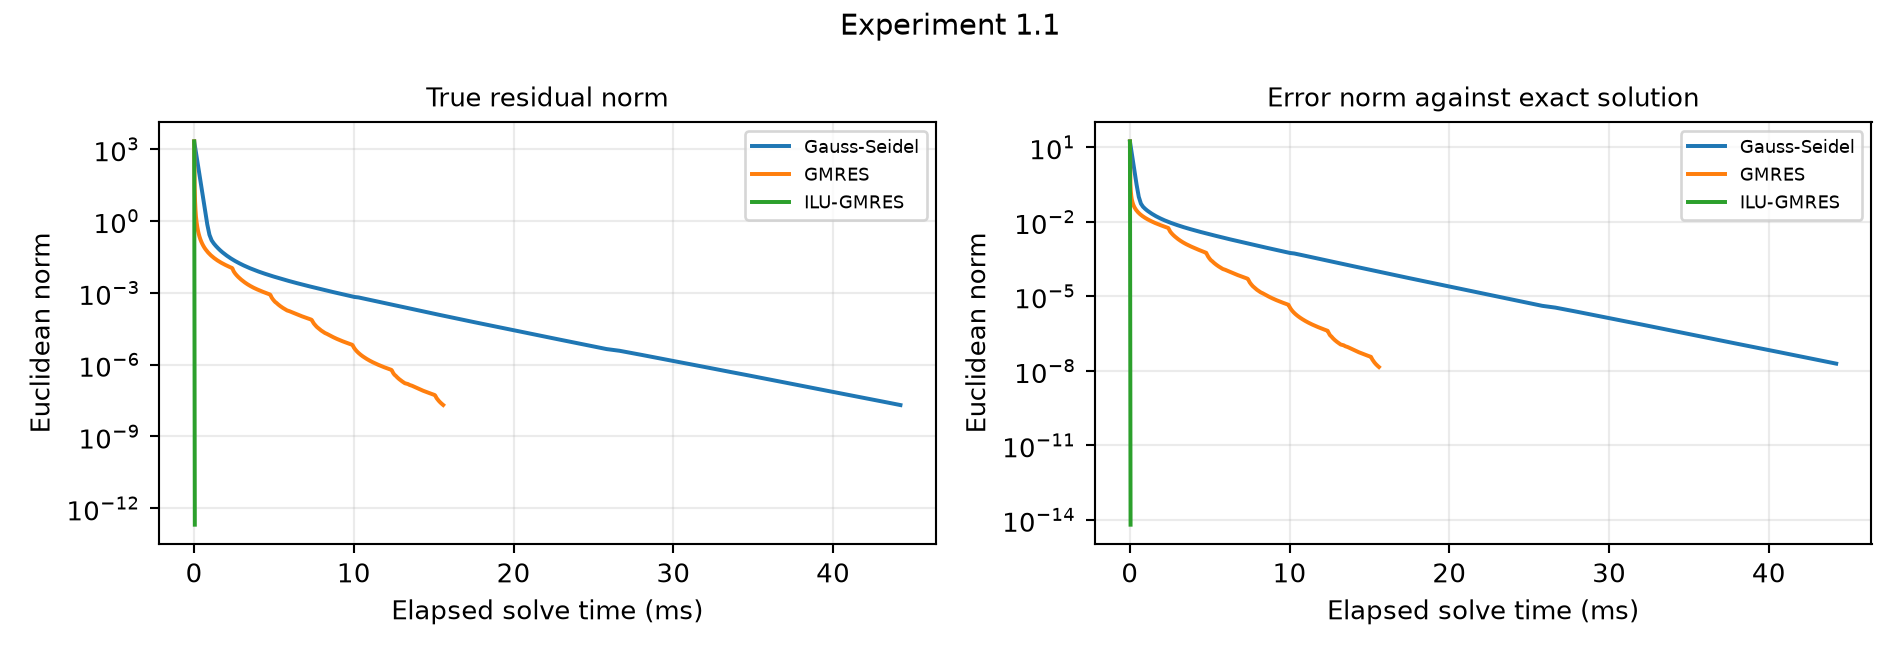
\includegraphics[width=\linewidth,height=58.419999999999995mm,keepaspectratio]{figures/1.1.png}\caption{Measured true residual and error against the prescribed exact solution versus elapsed solve time.}\end{figure}
ILU is essentially an exact factorization for this uncomplicated band structure and converges in one Krylov step. Its unusually small iteration count should not be generalized to arbitrary sparse systems. The absolute residual for unpreconditioned methods is around 2e-8 because the stopping condition is relative to the large right hand side.

\clearpage
\section*{3 Experiment 1.2 results}
Here n = 100. The diagonal is 1 through 100, both adjacent diagonals contain ones, and the two opposite corners equal 100. The displayed interior zeros and ellipses are interpreted as a cyclic tridiagonal pattern. The large corner in the first row removes diagonal dominance.

\[A_{ii}=i,\quad A_{i,i+1}=A_{i+1,i}=1,\quad A_{1,n}=A_{n,1}=n.\]
{\small\begin{tabular}{p{0.182\linewidth}p{0.182\linewidth}p{0.182\linewidth}p{0.182\linewidth}p{0.182\linewidth}}\toprule
Method & Iterations & Relative residual & Error norm & Total ms\\\midrule
Gauss-Seidel & 7 & 1.639e+13 & 1.572e+14 & 0.9810\\
GMRES & 91 & 9.227e-12 & 2.767e-09 & 7.0558\\
ILU-GMRES & 2 & 1.310e-14 & 1.945e-12 & 0.1317\\
\bottomrule\end{tabular}}\par
\begin{figure}[H]\centering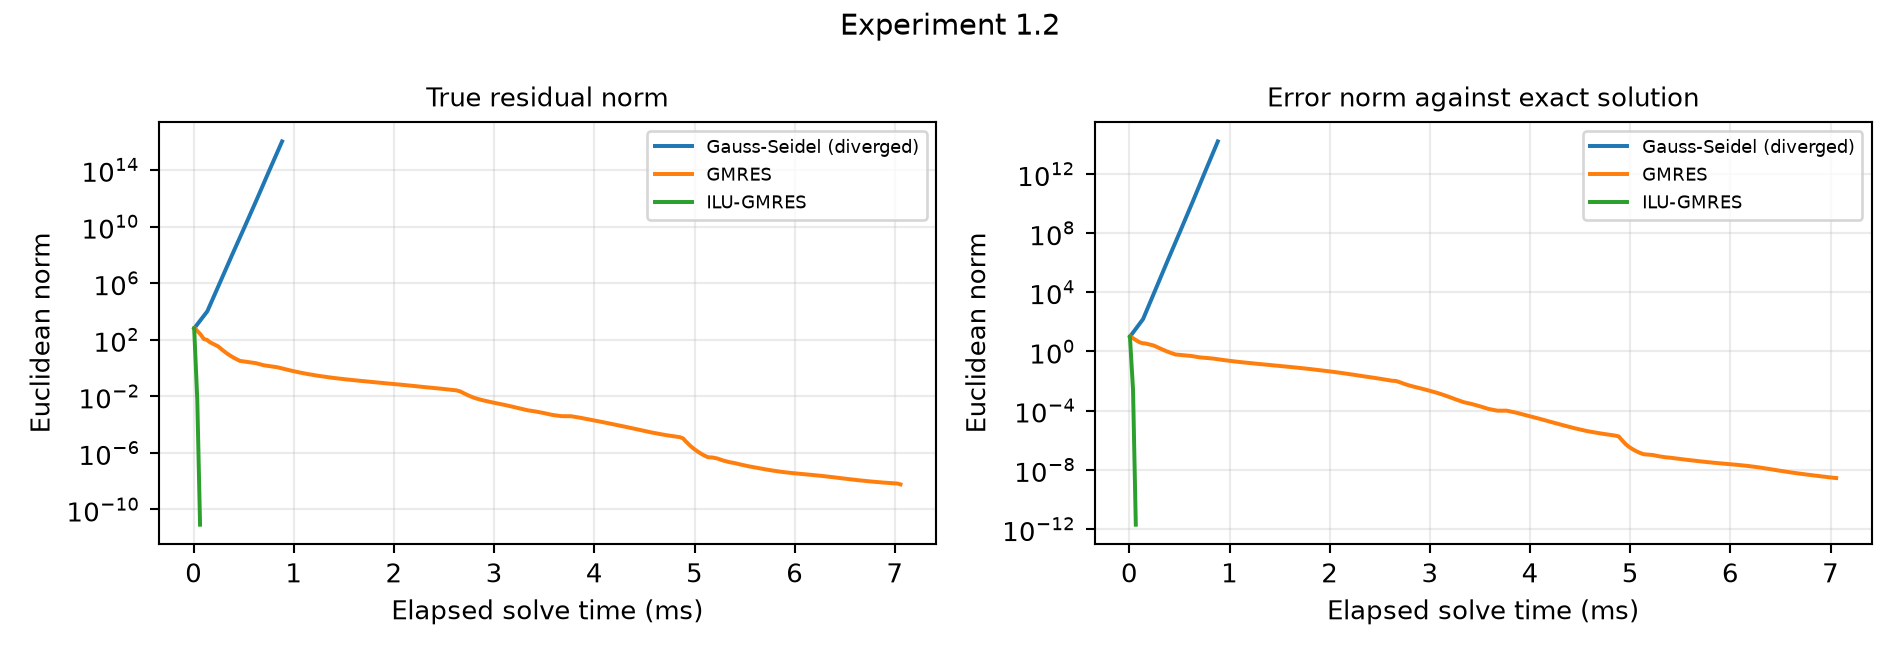
\includegraphics[width=\linewidth,height=58.419999999999995mm,keepaspectratio]{figures/1.2.png}\caption{Measured true residual and error against the prescribed exact solution versus elapsed solve time.}\end{figure}
Gauss Seidel triggers the divergence guard after seven sweeps; its large terminal residual is not a converged answer. GMRES and ILU GMRES meet the same residual criterion. The existence of a solution does not guarantee convergence of a stationary splitting. The figure retains the failed trajectory so the comparison does not hide the unstable method.

\clearpage
\section*{4 Experiment 1.3 results}
The printed ellipses are interpreted as constant bands: diagonal 4, adjacent diagonals 2, second adjacent diagonals 1, and a third lower diagonal of 1. The two unusual printed entries A(2,n) = 2 and A(n,2) = 3 are retained. All unspecified entries are zero. This explicit convention is essential because a different completion of the ellipses defines a different problem.

\[A_{ii}=4,\quad A_{i,i\pm1}=2,\quad A_{i,i\pm2}=1,\quad A_{i,i-3}=1.\]
{\small\begin{tabular}{p{0.182\linewidth}p{0.182\linewidth}p{0.182\linewidth}p{0.182\linewidth}p{0.182\linewidth}}\toprule
Method & Iterations & Relative residual & Error norm & Total ms\\\midrule
Gauss-Seidel & 119 & 9.704e-12 & 2.684e-09 & 16.2934\\
GMRES & 61 & 9.756e-12 & 8.226e-10 & 4.6607\\
ILU-GMRES & 3 & 3.547e-16 & 6.116e-15 & 0.2514\\
\bottomrule\end{tabular}}\par
\begin{figure}[H]\centering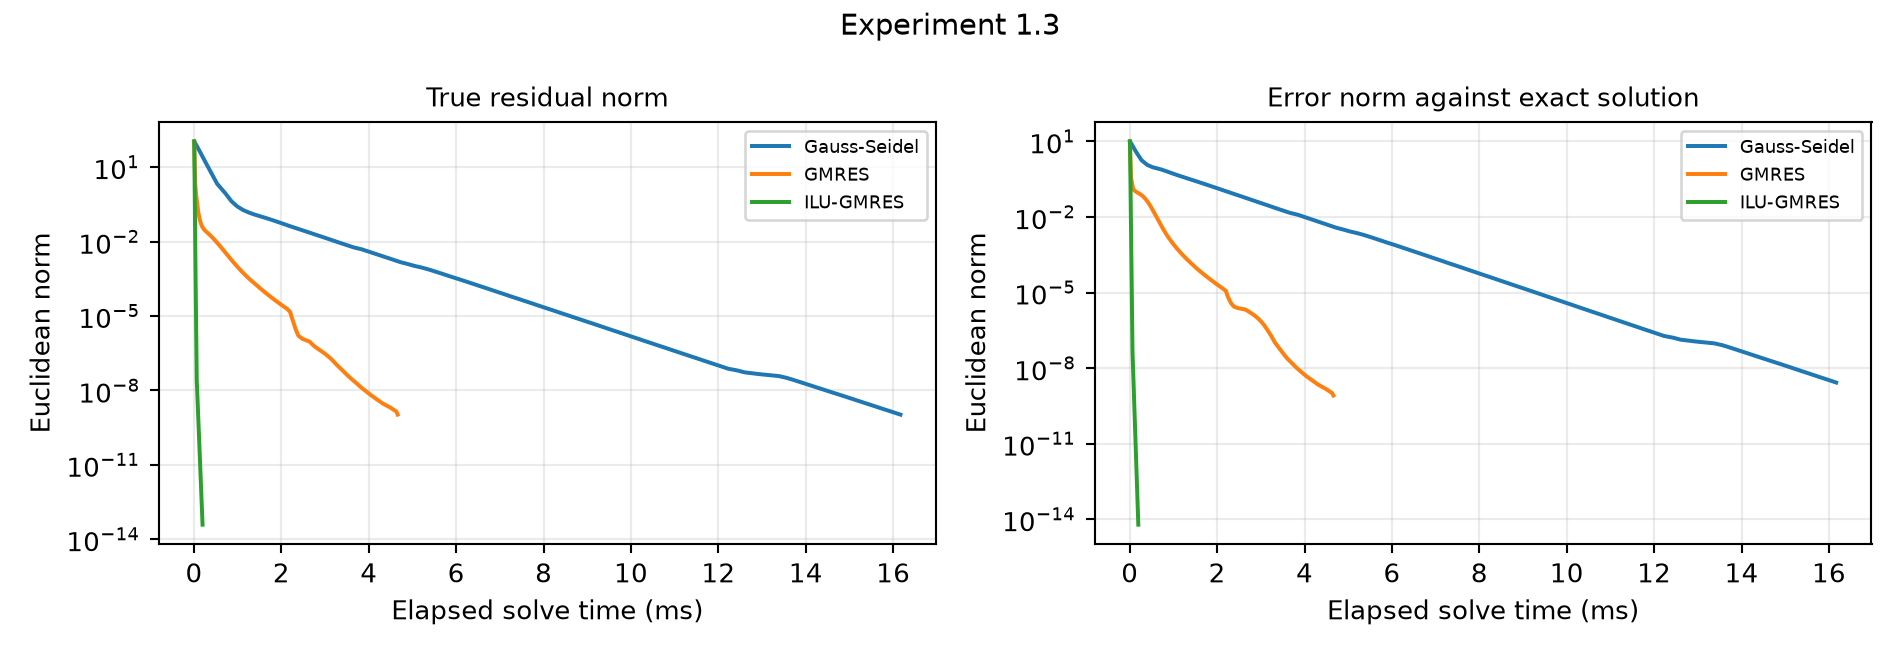
\includegraphics[width=\linewidth,height=58.419999999999995mm,keepaspectratio]{figures/1.3.png}\caption{Measured true residual and error against the prescribed exact solution versus elapsed solve time.}\end{figure}
The matrix is nonsymmetric under the stated band and corner convention. Gauss Seidel converges here even though strict diagonal dominance is unavailable as a sufficient test. ILU reduces the Krylov iteration count from 61 to 3. Agreement with the sparse direct solution and the all ones exact vector checks the actual assembled system.

\clearpage
\section*{5 Boundary value problem and discretization}
The handout supplies the exact solution u(x) = exp(x) + cos(pi x), endpoints u(0) = 2 and u(1) = e - 1, and an equation whose leading derivative is read as differentiation with respect to x. This is confirmed by substitution of the supplied exact solution and forcing.

\[u^{\prime\prime}-(1+x)^2u^{\prime}-e^{-x}u=f(x),\qquad 0<x<1.\]
\[f(x)=[1-(1+x)^2]e^x-\pi^2\cos(\pi x)+\pi(1+x)^2\sin(\pi x)-1-e^{-x}\cos(\pi x).\]
Let h = 1/N and x\_i = i h. Centered second and first differences have truncation error of order h squared for this smooth solution. Multiplication by 2 h squared gives the displayed tridiagonal system.

\[(2+hp_i)u_{i-1}-(4+2h^2e^{-x_i})u_i+(2-hp_i)u_{i+1}=2h^2f(x_i),\quad p_i=(1+x_i)^2.\]
\[F_1=2h^2f(x_1)-(2+hp_1)\,2.\]
\[F_{N-1}=2h^2f(x_{N-1})-(2-hp_{N-1})(e-1).\]
Only the N - 1 interior values are unknown. The boundary contributions are moved to the right hand side with a minus sign. The exact endpoints are reattached for the full grid. The sparse matrices, right hand sides, exact interior vectors and computed solutions are saved so the indexing and boundary correction can be audited.

\[E_\infty=\max_{1\leq i<N}|u_i-u(x_i)|,\qquad E_{2,h}=\left(h\sum_{i=1}^{N-1}|u_i-u(x_i)|^2\right)^{1/2}.\]
These grid errors compare with the continuous exact solution and therefore include discretization error. A separate direct solution of the same discrete system isolates the algebraic reference. Small residual alone does not imply equally small error, especially as conditioning worsens with mesh refinement.

\clearpage
\section*{6 Boundary value results and convergence}
{\small\begin{tabular}{p{0.12485714285714286\linewidth}p{0.12485714285714286\linewidth}p{0.12485714285714286\linewidth}p{0.12485714285714286\linewidth}p{0.12485714285714286\linewidth}p{0.12485714285714286\linewidth}p{0.12485714285714286\linewidth}}\toprule
N & Method & Steps & Rel res & Max error & L2 h error & Total ms\\\midrule
50 & GMRES & 298 & 9.64e-12 & 4.97357e-04 & 3.28999e-04 & 20.615\\
50 & ILU-GMRES & 1 & 7.72e-16 & 4.97356e-04 & 3.28998e-04 & 0.102\\
100 & GMRES & 915 & 1.00e-11 & 1.24310e-04 & 8.22306e-05 & 66.928\\
100 & ILU-GMRES & 1 & 1.09e-15 & 1.24307e-04 & 8.22284e-05 & 0.074\\
200 & GMRES & 3207 & 9.95e-12 & 3.10840e-05 & 2.05623e-05 & 246.550\\
200 & ILU-GMRES & 1 & 1.86e-15 & 3.10747e-05 & 2.05558e-05 & 0.102\\
\bottomrule\end{tabular}}\par
\begin{figure}[H]\centering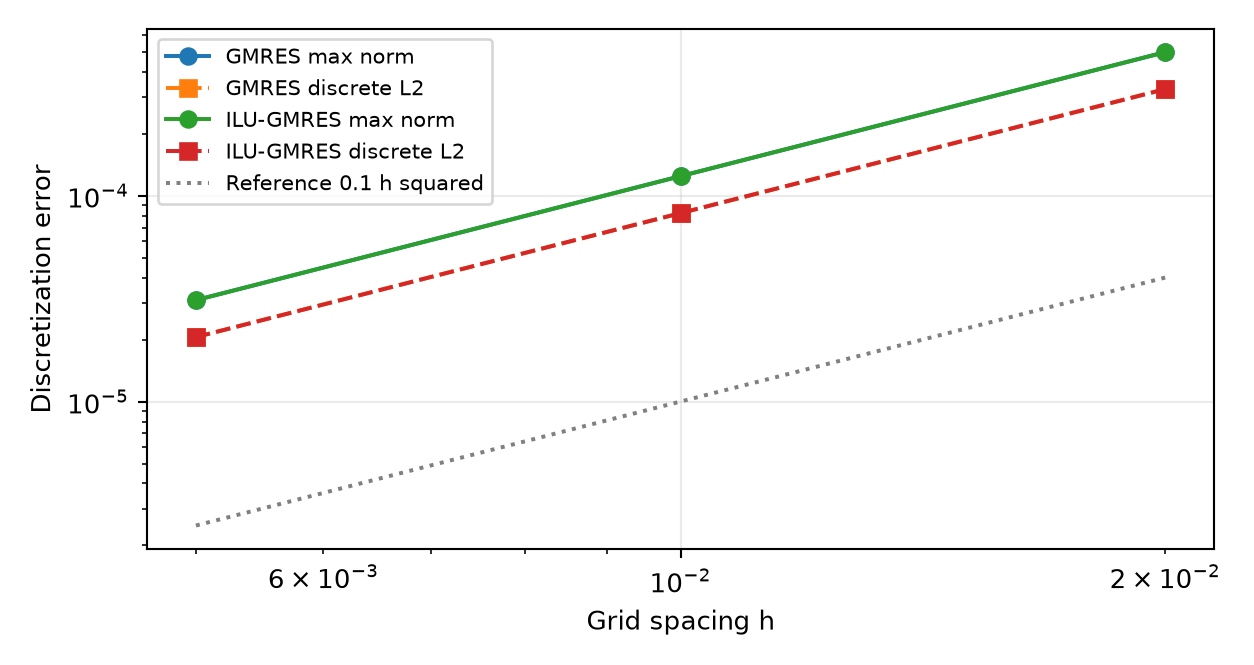
\includegraphics[width=\linewidth,height=63.5mm,keepaspectratio]{figures/convergence.png}\caption{Grid error decreases quadratically as h is halved. Curves of both solvers nearly coincide.}\end{figure}
GMRES maximum norm observed orders are 2.000338, 1.999697. The order is computed as log base two of consecutive error ratios. Both norms and both solvers give approximately second order convergence.

ILU-GMRES maximum norm observed orders are 2.000371, 2.000093. The order is computed as log base two of consecutive error ratios. Both norms and both solvers give approximately second order convergence.

The ILU solve takes one Krylov step for each tridiagonal grid system. Unpreconditioned iteration counts grow strongly under refinement. Because the algebraic tolerance is sufficiently small, further residual reduction does not materially improve the leading finite difference error.

\clearpage
\section*{7 Boundary value iteration histories}
\begin{figure}[H]\centering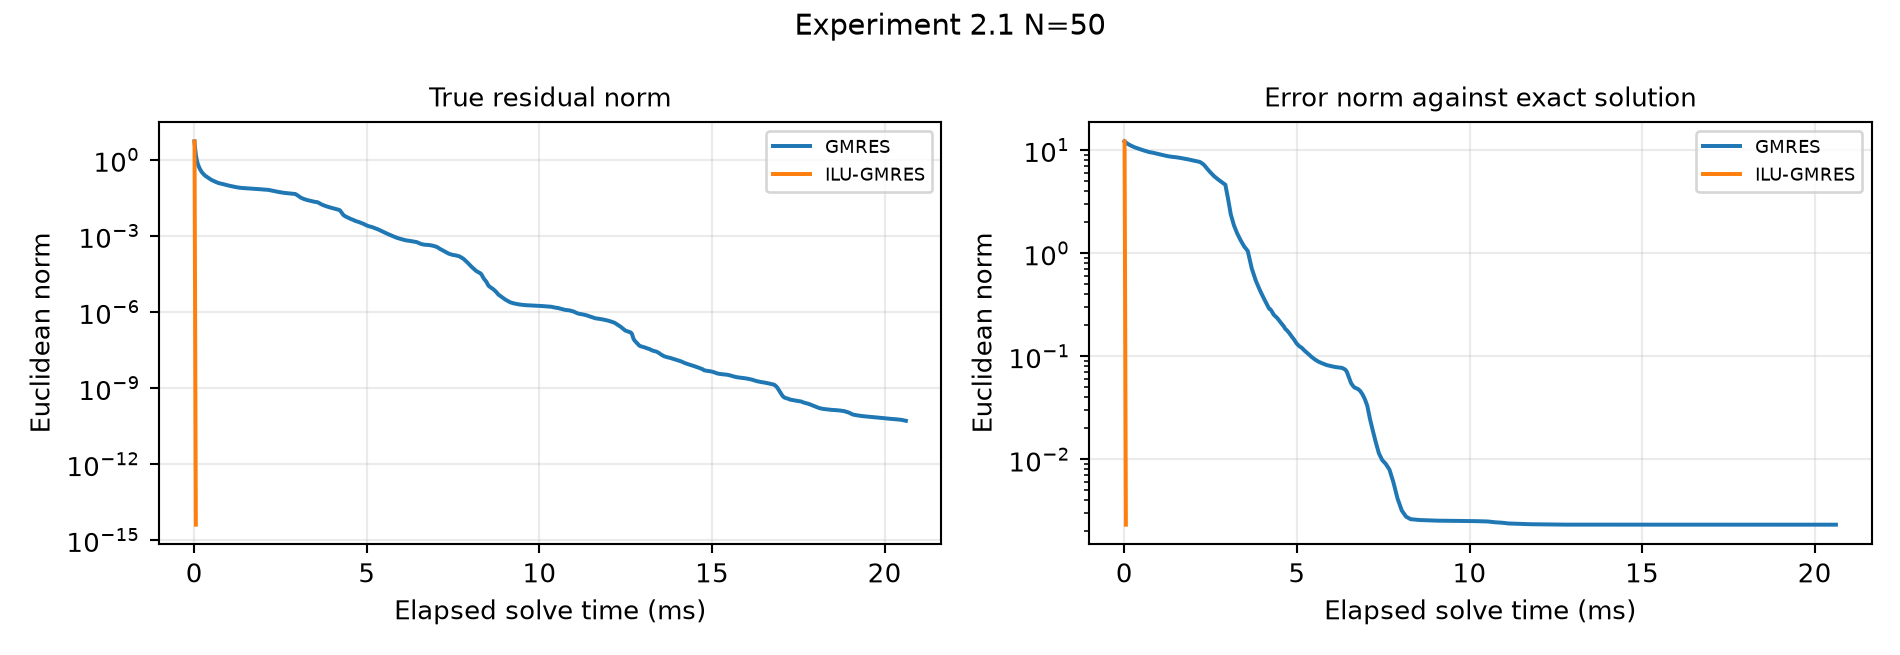
\includegraphics[width=\linewidth,height=44.449999999999996mm,keepaspectratio]{figures/2.1_N_50.png}\caption{N = 50: residual and Euclidean grid error against the continuous exact solution.}\end{figure}
\begin{figure}[H]\centering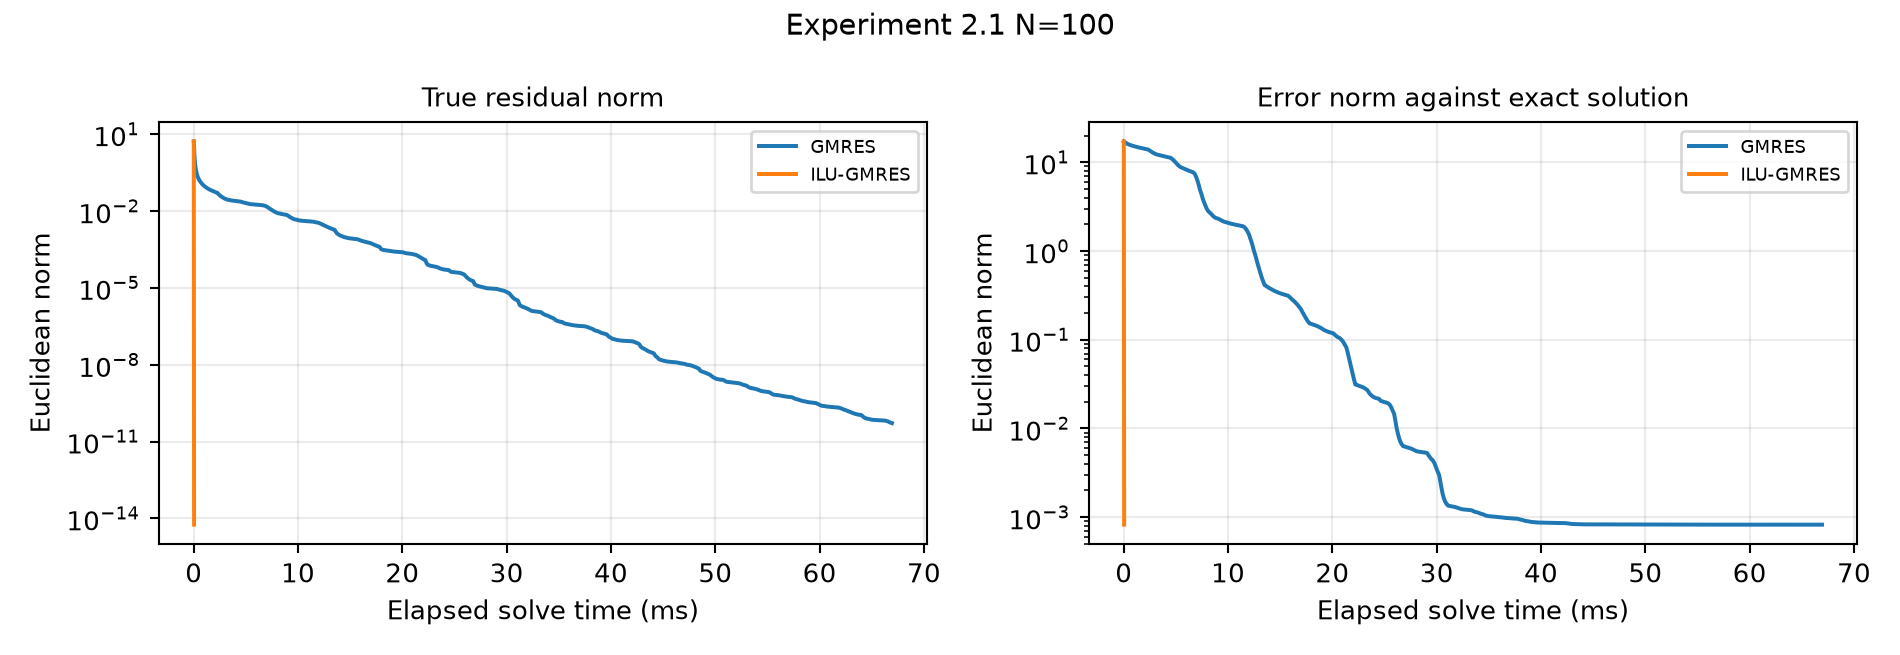
\includegraphics[width=\linewidth,height=44.449999999999996mm,keepaspectratio]{figures/2.1_N_100.png}\caption{N = 100: residual and Euclidean grid error against the continuous exact solution.}\end{figure}
\begin{figure}[H]\centering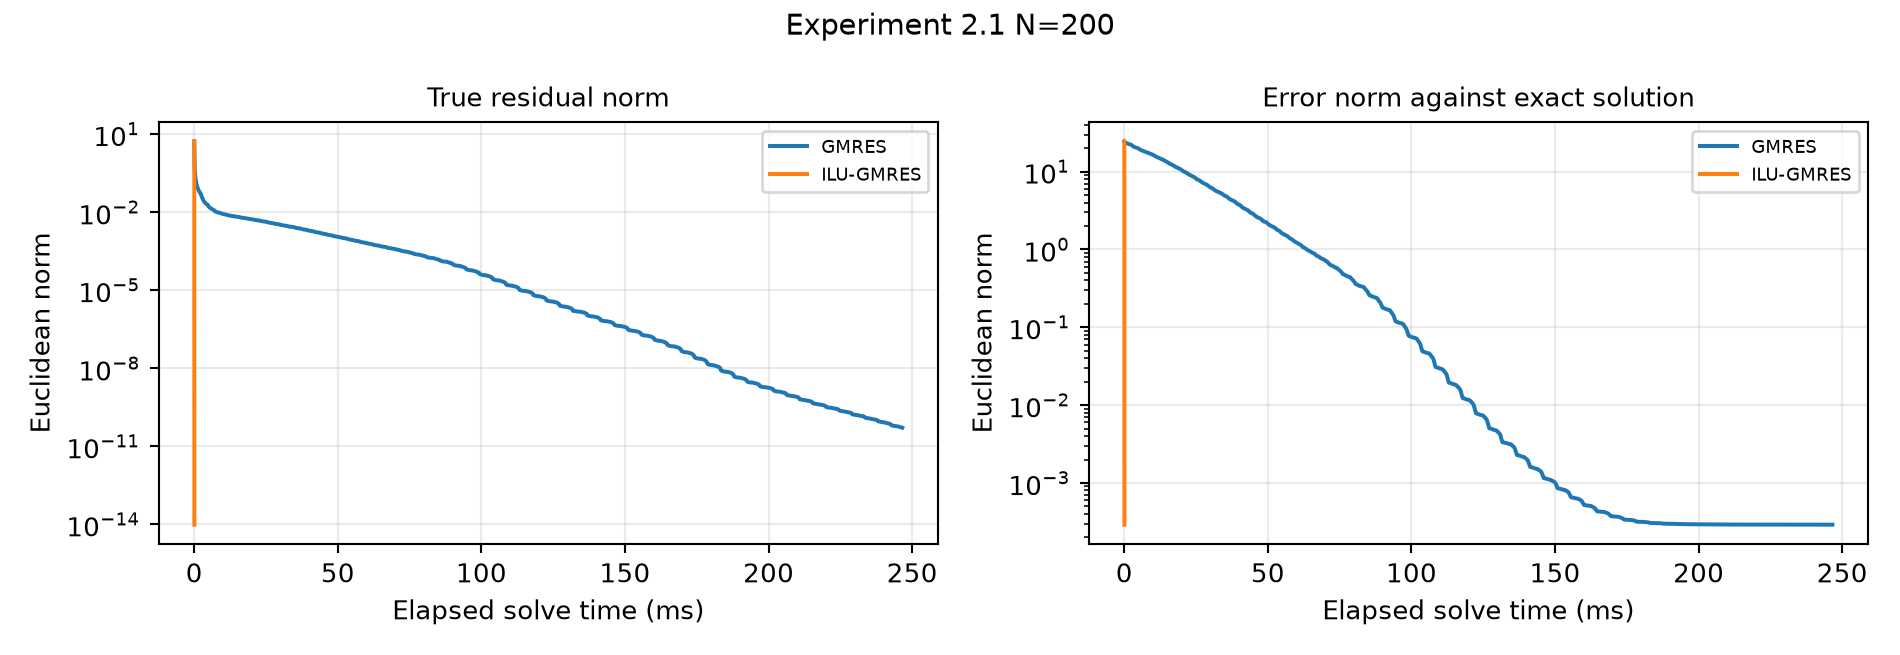
\includegraphics[width=\linewidth,height=44.449999999999996mm,keepaspectratio]{figures/2.1_N_200.png}\caption{N = 200: residual and Euclidean grid error against the continuous exact solution.}\end{figure}
A residual continues decreasing after the grid error approaches the discretization floor. The error need not decrease monotonically because GMRES minimizes the residual in its search space, not the error against the continuous solution. ILU setup is excluded from the horizontal axes but included in total time tables.

\clearpage
\section*{8 Verification and reproduction}
The numerical verification script passes 10 of 10 checks covering case coverage, direct residuals, the expected divergence, solver convergence, SciPy agreement, time history consistency, and second order grid convergence in both norms. A separate delivery audit checks saved solutions against their sparse matrices and right hand sides.

{\small\begin{tabular}{p{0.482\linewidth}p{0.482\linewidth}}\toprule
Environment & Recorded value\\\midrule
python & 3.13.7\\
numpy & 2.5.3\\
scipy & 1.18.1\\
machine & arm64\\
platform & macOS-27.0-arm64-arm-64bit-Mach-O\\
\bottomrule\end{tabular}}\par
From the package root, run python reproduce.py to regenerate numerical results, verification, figures, report content, the LaTeX PDF and the editable Word document. See README.md for the individual commands and directory layout. The final PDF is compiled from LaTeX before Word generation; the Word document uses native editable Office equations.

The implementation records true residuals explicitly and cross checks SciPy GMRES with its own interface. A mismatch in iteration counts between left and right preconditioning is not itself a contradiction. Timings are measured locally and include instrumentation overhead; no claim is made about device deployment or production solver performance.

Source: the supplied two page course handout, preserved byte for byte in source. Experiment 1.3 uses the explicit band completion stated in Section 4; the derivative variable in the boundary value problem is taken as x to match the supplied exact solution. These are the only transcription conventions affecting the numerical model.

\end{document}